\documentclass[presentation]{beamer}
\mode<presentation>
% grise les zones en pause
{\setbeamercovered{transparent}}

%l'option 'handout' pour imprimer sans les pauses
%\documentclass[handout]{beamer}

% Beamer style
%\usetheme[secheader]{Madrid}
\usetheme{CambridgeUS}
%\usetheme{Boadilla}
\usecolortheme[rgb={0.65,0.15,0.25}]{structure}
%\usefonttheme[onlymath]{serif}
\beamertemplatenavigationsymbolsempty
%\AtBeginSubsection

% Packages
%\usepackage[french]{babel}
\usepackage[latin1]{inputenc}
\usepackage{color}
%\usepackage{dsfont, stmaryrd}
\usepackage{amsmath, amsfonts, amssymb}
\usepackage{epsfig}
\usepackage{url}
\usepackage{/home/robin/LATEX/astats}
%\usepackage[all]{xy}
\usepackage{graphicx}

% Commands
\definecolor{darkred}{rgb}{0.65,0.15,0.25}
%\newcommand{\emphase}[1]{\textcolor{darkred}{#1}}
\newcommand{\emphase}[1]{{#1}}
\newcommand{\paragraph}[1]{\textcolor{darkred}{#1}}
\newcommand{\refer}[1]{{\footnotesize{\textcolor{gray}{{[\cite{#1}]}}}}}
\newcommand{\Refer}[1]{{\footnotesize{\textcolor{gray}{[{\sl #1}]}}}}
\newcommand{\newblock}{}

% Symbols
\newcommand{\Abf}{{\bf A}}
\newcommand{\Beta}{\text{B}}
\newcommand{\Bcal}{\mathcal{B}}
\newcommand{\BIC}{\text{BIC}}
\newcommand{\Ccal}{\mathcal{C}}
\newcommand{\dd}{\text{~d}}
\newcommand{\dbf}{{\bf d}}
\newcommand{\Dcal}{\mathcal{D}}
\newcommand{\Esp}{\mathbb{E}}
\newcommand{\Ebf}{{\bf E}}
\newcommand{\Ecal}{\mathcal{E}}
\newcommand{\Gcal}{\mathcal{G}}
\newcommand{\Gam}{\mathcal{G}\text{am}}
\newcommand{\Hcal}{\mathcal{H}}
\newcommand{\Ibb}{\mathbb{I}}
\newcommand{\Ibf}{{\bf I}}
\newcommand{\ICL}{\text{ICL}}
\newcommand{\Cov}{\mathbb{C}\text{ov}}
\newcommand{\Corr}{\mathbb{C}\text{orr}}
\newcommand{\Var}{\mathbb{V}}
\newcommand{\Vsf}{\mathsf{V}}
\newcommand{\pen}{\text{pen}}
\newcommand{\Fcal}{\mathcal{F}}
\newcommand{\Hbf}{{\bf H}}
\newcommand{\Jcal}{\mathcal{J}}
\newcommand{\Kbf}{{\bf K}}
\newcommand{\Lcal}{\mathcal{L}}
\newcommand{\Mcal}{\mathcal{M}}
\newcommand{\mbf}{{\bf m}}
\newcommand{\mum}{\mu(\mbf)}
\newcommand{\Ncal}{\mathcal{N}}
\newcommand{\Nbf}{{\bf N}}
\newcommand{\Nm}{N(\mbf)}
\newcommand{\Ocal}{\mathcal{O}}
\newcommand{\Obf}{{\bf 0}}
\newcommand{\Omegas}{\underset{s}{\Omega}}
\newcommand{\Pbf}{{\bf P}}
\newcommand{\Pcal}{\mathcal{P}}
\newcommand{\Qcal}{\mathcal{Q}}
\newcommand{\Rbb}{\mathbb{R}}
\newcommand{\Rcal}{\mathcal{R}}
\newcommand{\Scal}{\mathcal{S}}
\newcommand{\Ucal}{\mathcal{U}}
\newcommand{\Vcal}{\mathcal{V}}
\newcommand{\BP}{\text{BP}}
\newcommand{\EM}{\text{EM}}
\newcommand{\VEM}{\text{VEM}}
\newcommand{\VBEM}{\text{VBEM}}
\newcommand{\cst}{\text{cst}}
\newcommand{\obs}{\text{obs}}
\newcommand{\ra}{\emphase{\mathversion{bold}{$\rightarrow$}~}}
%\newcommand{\transp}{\text{{\tiny $\top$}}}
\newcommand{\transp}{\text{{\tiny \mathversion{bold}{$\top$}}}}

% Directory
\newcommand{\figmixt}{/home/robin/ENSEIGN/COURS/MELANGE}
\newcommand{\figbma}{/home/robin/RECHERCHE/RUPTURES/MELANGE/Exemples/Grippe}
\newcommand{\fignet}{../FIGURES}
\newcommand{\figeco}{/home/robin/RECHERCHE/ECOLOGIE/EXPOSES/FIGURES}
%\newcommand{\figmotif}{/home/robin/RECHERCHE/RESEAUX/Motifs/FIGURES}


%--------------------------------------------------------------------
%--------------------------------------------------------------------

%--------------------------------------------------------------------
%--------------------------------------------------------------------
\begin{document}
%--------------------------------------------------------------------
%--------------------------------------------------------------------

%--------------------------------------------------------------------
\title[Heterogeneity in interaction networks]{Deciphering and modeling heterogeneity \\
in
interaction networks\\ {\large (using variational approximations)}}

\author{S. Robin}

\institute[INRA / AgroParisTech]{INRA / AgroParisTech \\
  \vspace{-.25\textheight}
  \begin{center}
  \begin{tabular}{ccccc}
    
\includegraphics[width=2.5cm]{\fignet/LogoINRA-Couleur} & 
    \hspace{.5cm} &
    
\includegraphics[width=3.75cm]{\fignet/logagroptechsolo} & 
    \hspace{.5cm} &
    
\includegraphics[width=2.5cm]{\fignet/logo-ssb}
    \\ 
  \end{tabular} 
  \end{center}
  \medskip
  }

\date[MMCS'13]{Mathematical Modeling of Complex Systems \\
  December 2013, Ecole Centrale de Paris}

%--------------------------------------------------------------------
%--------------------------------------------------------------------
\maketitle
%--------------------------------------------------------------------

%--------------------------------------------------------------------
\frame{\frametitle{Outline}
  \tableofcontents
  }
%--------------------------------------------------------------------

% Bayesian model averaging (with Volant, Martin)
% * BMA
% * Variational weights 
% 
% Towards graphon estimation (with Latouche)
% * Connexion between SBM and graphon 
% * BMA for SBM for graphon
% * French political blogosphere

%--------------------------------------------------------------------
%--------------------------------------------------------------------
\section[State-space models for networks]{State-space models for networks (inc. SBM)}
%--------------------------------------------------------------------
\subsection*{Heterogeneity in networks}
\frame{\frametitle{Heterogeneity in interaction networks}}
%--------------------------------------------------------------------

%--------------------------------------------------------------------
\frame{\frametitle{Understanding network structure}

  Networks describe interactions between entities. \\
  ~\\
  Observed networks display heterogeneous topologies, that one would like to decipher and better understand. \\
  ~\\

  \onslide+<2->{
    \begin{tabular}{ll}
    %\hspace{-.5cm}
    \begin{tabular}{p{.5\textwidth}}
      \paragraph{Dolphine social network.} \\
      %\epsfig{file=../Figures/NeG04-Fig11.ps, clip=, width=.5\textwidth}
      \includegraphics[width=.4\textwidth]{../FIGURES/NeG04-Fig11} \\
      \refer{NeG04}
    \end{tabular}
    & 
    \hspace{-.5cm}
    \begin{tabular}{p{.5\textwidth}}
      \paragraph{Hyperlink network.} \\
      \includegraphics[width=.4\textwidth]{../FIGURES/NeG04-Fig13} 
    \end{tabular} 
  \end{tabular} 
  }
  
  }

%--------------------------------------------------------------------
\frame{\frametitle{Modelling network heterogeneity}

  \paragraph{Latent variable models} allow to capture
  the underlying structure of a network.

  \bigskip \bigskip \pause
  \paragraph{General setting for binary graphs.} \refer{BJR07}: %\pause
  \begin{itemize}
   \item   \emphase{A latent (unobserved) variable $Z_i$} is associated with each node:
  $$
  \{Z_i\} \text{ iid } \sim \pi 
  $$
  \item 
  Edges \emphase{$Y_{ij} = \Ibb\{i \sim j\}$ are independent conditionally} to the $Z_i$'s:
  $$
  \{Y_{ij}\} \text{ independent } | \{Z_i\}: \Pr\{Y_{ij} = 1\} = \gamma(Z_i, Z_j)
  $$
  \end{itemize}

  \bigskip \pause
  \paragraph{We focus here on model approaches}, in contrast with, e.g.
  \begin{itemize}
  \item Graph clustering \refer{GiN02}, \refer{New04}; 
  \item Spectral clustering \refer{LBB08}.
  \end{itemize}

  }

%--------------------------------------------------------------------
\subsection*{State space models}
%--------------------------------------------------------------------
\frame{\frametitle{Latent space models}

  \vspace{-.2\textheight}
  \begin{tabular}{cc}
  \vspace{-.3\textheight}
  \hspace{-.05\textwidth}
    \begin{tabular}{p{.5\textwidth}}
      \onslide+<1->{
	\paragraph{State-space model: principle.}}
	 \begin{itemize}
	   \onslide+<2->{
        \item Consider $n$ nodes ($i = 1..n$); \\ ~ } 
        \onslide+<3->{
        \item $Z_i = $ unobserved position of node $i$, e.g.
          $$
          \{Z_i\} \text{ iid } \sim \Ncal(0 ,I)
          $$} 
        \onslide+<4->{
        \item Edge $\{Y_{ij}\}$ independent given $\{Z_i\}$, e.g.
          $$
          \Pr\{Y_{ij} = 1\} = \gamma(Z_i, Z_j)
          $$
          $\gamma(z, z') = f(||z - z'||)$.}
      \end{itemize}
    \end{tabular}
    & 
    \hspace{-.05\textwidth}
    \begin{tabular}{p{.5\textwidth}}
      \vspace{1cm}
      \begin{overprint}
        \onslide<3>
        \hspace{-.1\textwidth}
        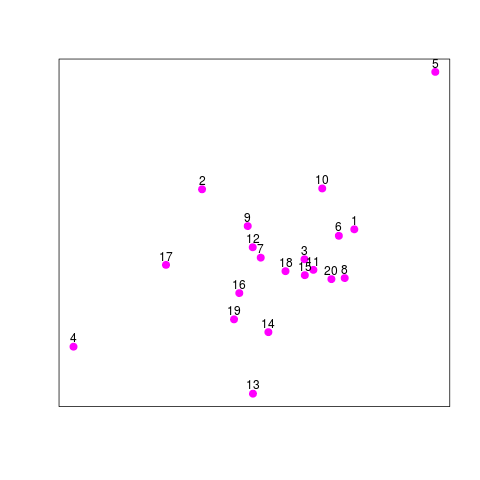
\includegraphics[width=.5\textwidth]{\fignet/FigCLADAG-LPM-Y}    
        \onslide<4>
        \hspace{-.1\textwidth}
        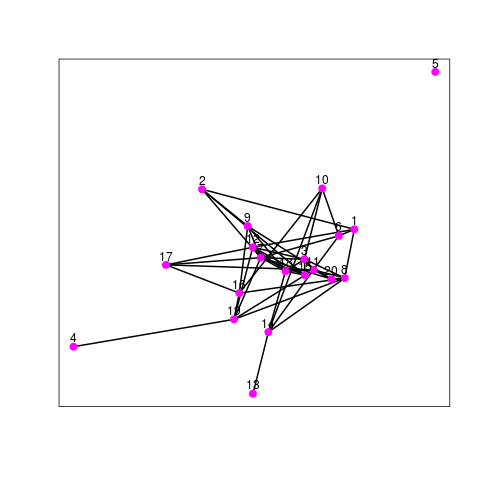
\includegraphics[width=.5\textwidth]{\fignet/FigCLADAG-LPM-XY}    
        \onslide<5>
%         \hspace{-.1\textwidth}
%         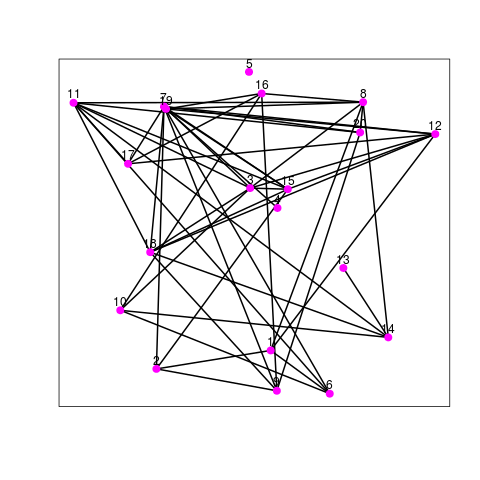
\includegraphics[width=.5\textwidth]{\fignet/FigCLADAG-LPM-X1}    
%         \onslide<6>
%         \hspace{-.1\textwidth}
%         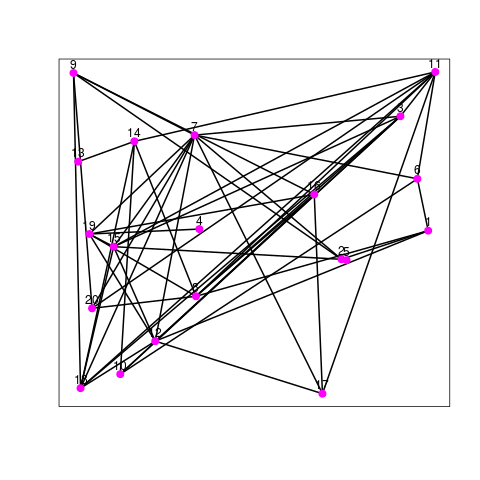
\includegraphics[width=.5\textwidth]{\fignet/FigCLADAG-LPM-X2}    
%         \onslide<7>
        $
        Y = \left( {\footnotesize
		\begin{array}{cccccc}
		0 & 1 & 1 & 0 & 1 & \dots \\
		0 & 0 & 1 & 0 & 1 & \dots \\
		0 & 0 & 0 & 0 & 0 & \dots \\
		0 & 0 & 0 & 0 & 1 & \dots \\
		0 & 0 & 0 & 0 & 0 & \dots \\
		\vdots & \vdots & \vdots & \vdots & \vdots & \ddots  
		\end{array}
        } \right)
        $
      \end{overprint}
    \end{tabular}
  \end{tabular}
  }

%--------------------------------------------------------------------
\frame{\frametitle{A variety of state-space models}

  \bigskip%\pause
  \paragraph{Continuous.} Latent position models.
  \begin{itemize}
   \item \refer{HRH02}: 
   $$
   Z_i \in \Rbb^d, \qquad \text{logit}[\gamma(z, z')] = a - |z-z'|
   $$
   \item \refer{HRT07}:
   $$
   Z_i \sim \sum_k p_k \Ncal_d(\mu_k, \sigma^2_k I)
   $$
   \item \refer{LoS06}:
   $$
   Z_i \sim \Ucal_{[0, 1]}, \qquad \gamma(z, z'): [0, 1]^2 \rightarrow [0, 1] =: \text{graphon function}
   $$
   \item \refer{DPV10}:
   $$
   Z_i \in \Scal_K, \qquad \gamma(z, z') = \sum_{k, \ell} z_k z'_\ell \gamma_{k\ell}
   $$
  \end{itemize}
%   %\bigskip%\pause
%   \paragraph{Discrete.} Hidden class models. 
%   \begin{itemize}
%    \item \refer{NoS01}:
%    $$
%    Z_i \in \{1, \dots, K\}, \qquad \gamma(k, \ell) = \gamma_{k\ell}.   
%    $$
%   \end{itemize}
  }

%--------------------------------------------------------------------
\frame{\frametitle{Stochastic Block Model (SBM)}

  \begin{tabular}{cc}
    \hspace{-.5cm}
    \begin{tabular}{p{.5\textwidth}}
      \onslide+<1->{
	\paragraph{A mixture model for random graphs.}} \refer{NoS01}
      \onslide+<2->{
	\begin{itemize}
        \item Consider $n$ nodes ($i = 1..n$); \\ ~ } 
        \onslide+<3->{
        \item $Z_i = $ unobserved label of node $i$:
          $$
          \{Z_i\} \text{ iid } \sim \Mcal(1; \pi)
          $$
          $\pi = (\pi_1, ... \pi_K)$; \\ ~ } 
        \onslide+<4->{
        \item Edge $Y_{ij}$ depends on the labels:
          $\{Y_{ij}\}$ independent given $\{Z_i\}$,
          $$
          \Pr\{Y_{ij} = 1\} = \gamma(Z_i, Z_j)
          $$}
      \end{itemize}
    \end{tabular}
    & 
    \hspace{-.5cm}
    \begin{tabular}{p{.5\textwidth}}
      \vspace{1cm}
      \begin{overprint}
        \onslide<2>
        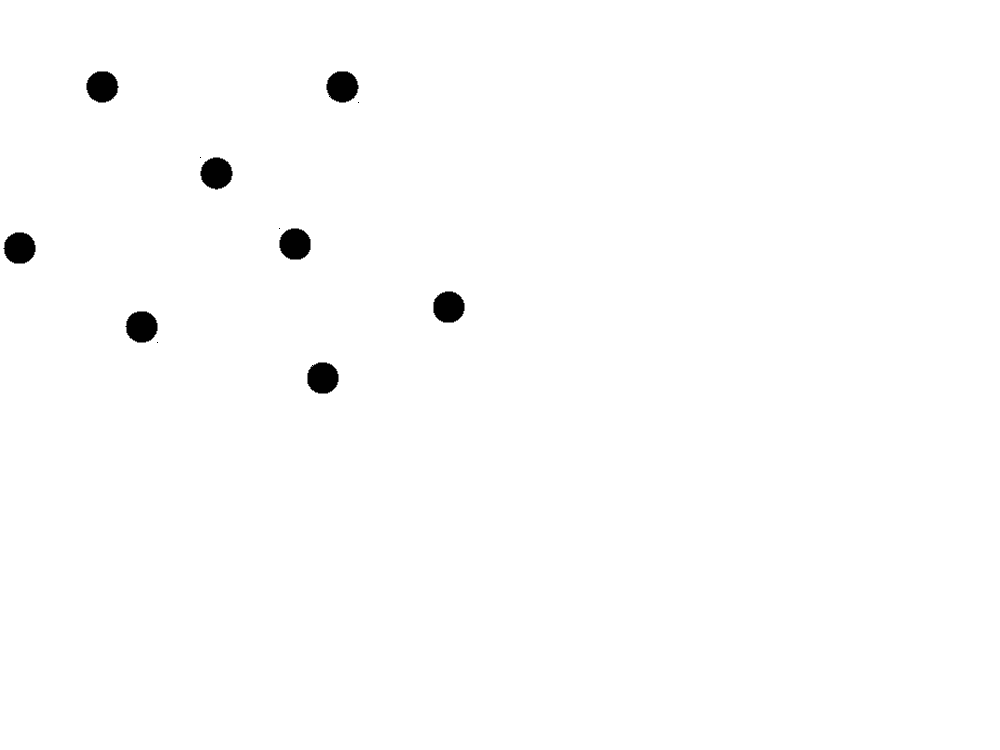
\includegraphics[width=.75\textwidth]{\fignet/FigSBM-Model-1}    
        \onslide<3>
        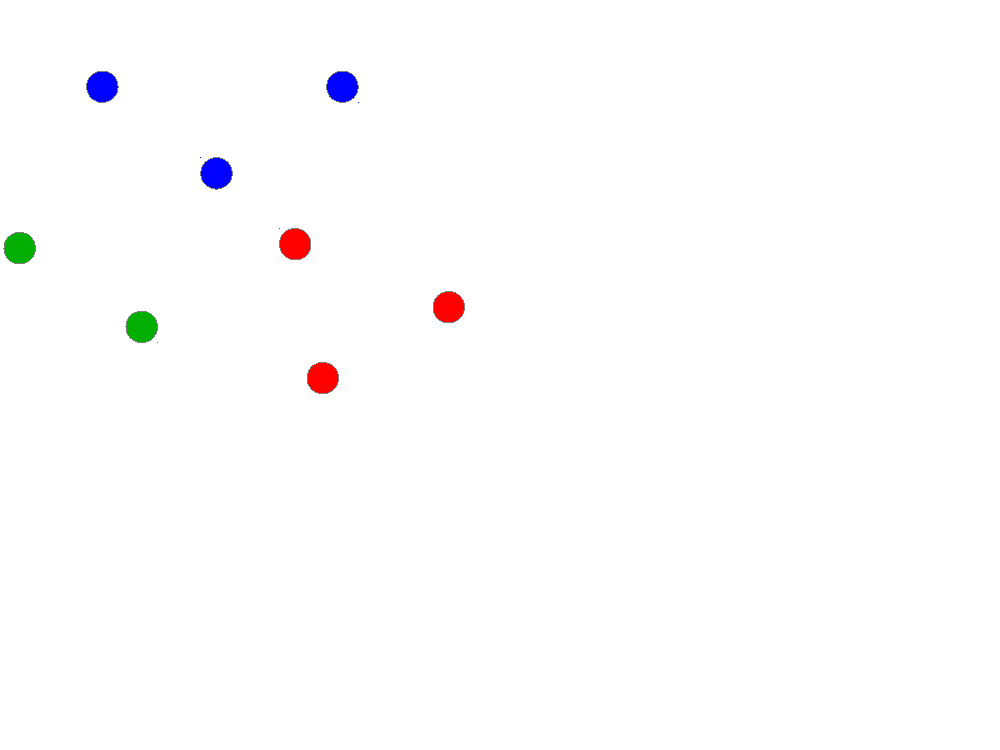
\includegraphics[width=.75\textwidth]{\fignet/FigSBM-Model-2}    
        \onslide<4>
        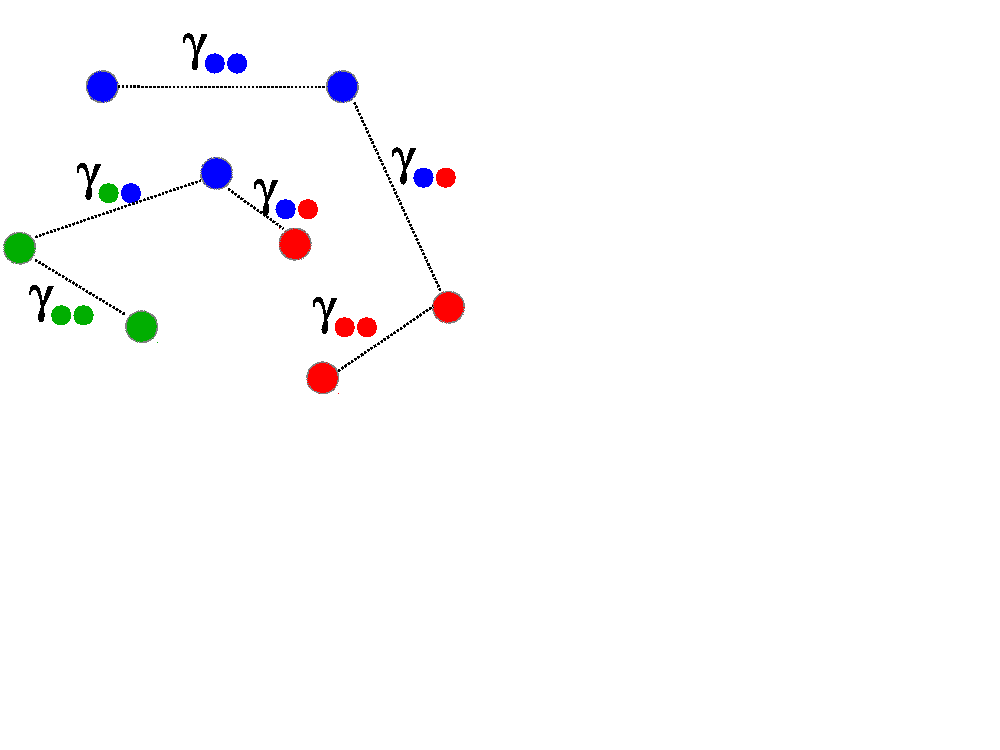
\includegraphics[width=.75\textwidth]{\fignet/FigSBM-Model-3}    
        \onslide<5>
        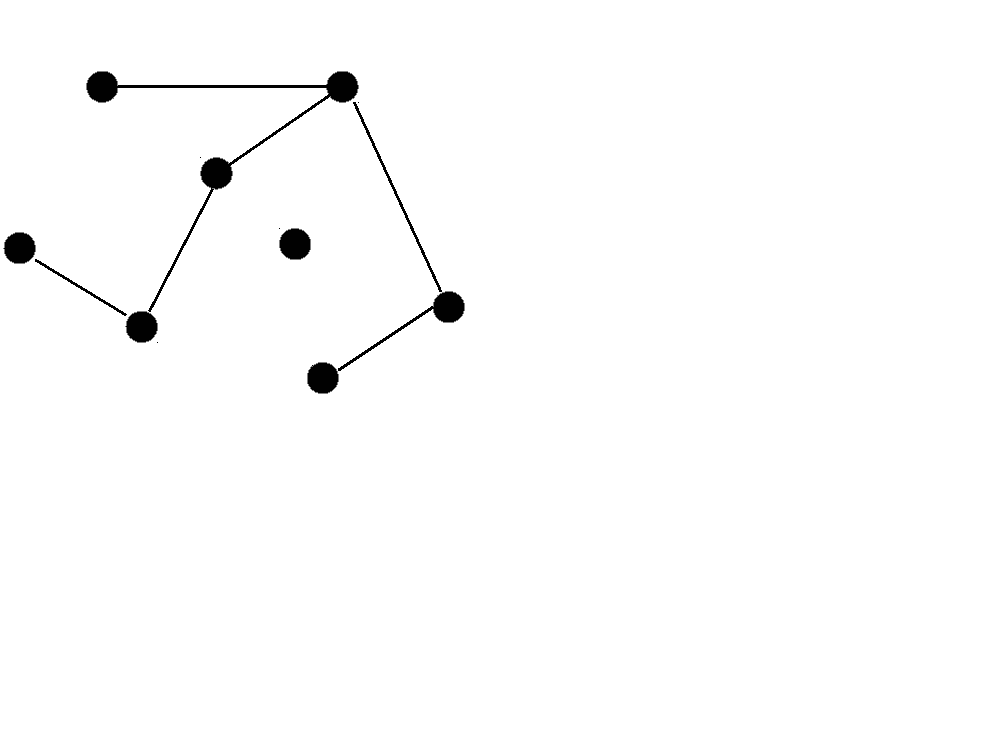
\includegraphics[width=.75\textwidth]{\fignet/FigSBM-Model-5}    
      \end{overprint}
    \end{tabular}
  \end{tabular}
  }

%--------------------------------------------------------------------
%--------------------------------------------------------------------
\section[Variational inference]{Variational inference (inc. SBM)}
\frame{\frametitle{Variational inference}

  Joint work with J.-J. Daudin, S. Gazal, F. Picard
  
  \bigskip \bigskip 
  \refer{DPR08}, \refer{GDR11}
}
%--------------------------------------------------------------------

%--------------------------------------------------------------------
\subsection*{Incomplete data models}
%--------------------------------------------------------------------
%--------------------------------------------------------------------
\frame{\frametitle{Incomplete data models}

	\paragraph{Aim.} Based on the observed network $Y = (Y_{ij})$, we want to infer
	\begin{itemize}
	\item the parameters
	$$
	\theta = (\pi, \gamma)
	$$
	\item the hidden states 
	$$
	Z = (Z_i)
	$$
	\end{itemize}

	\bigskip \bigskip \pause
	State space models belong to the class of incomplete data models as
	\begin{itemize}
	\item the edges $(Y_{ij})$ are observed,
	\item the latent positions (or status) $(Z_i)$ are not.
	\end{itemize}
	\ra usual issue in unsupervised classification.
}

%--------------------------------------------------------------------
\frame{\frametitle{Frequentist maximum likelihood inference}

  \paragraph{Likelihood.} The (log-)likelihood
  $$
  \log P(Y; \theta) = \log \sum_{Z} P(Y, Z; \theta)
  $$
  can not be computed.

  \pause\bigskip\bigskip
  \paragraph{EM trick.} But it can be decomposed as
  $$
  \log P(Y; \theta) = \log P(Y, Z; \theta) - \log
  P(Z | Y; \theta), 
  $$
  \pause the conditional expectation of which gives
  \begin{eqnarray*}
    \Esp[\log P(Y;\theta)|Y] & = & \Esp[\log P(Y, Z;
    \theta)|Y] - \Esp[\log P(Z | Y; \theta)|Y] \\ 
    \pause
    \log P(Y; \theta) & = & \Esp[\log P(Y, Z;
    \theta)|Y] + \Hcal[P(Z | Y; \theta)]
  \end{eqnarray*}
  where $\Hcal$ stands for the entropy.
  }

%--------------------------------------------------------------------
\frame{\frametitle{EM algorithm}

  Aims at maximizing the log-likelihood
  $$
  \log P(Y; \theta)
  $$
  through the alternation of two steps \refer{DLR77}
  
  \bigskip \pause 
  \paragraph{M-step:} maximize $\Esp[\log P(Y, Z;
    \theta)|Y]$ with respect to $\theta$ \\
    \ra generally similar to standard MLE. \\
  
  \bigskip \pause 
  \paragraph{E-step:} calculate $P(Z|Y)$ (at least, some moments) \\
  \pause \ra sometimes straightforward (independent mixture models: Bayes formula) \\
  \pause \ra sometimes tricky but doable (HMMs: forward-backward recursion) \\
  \pause \ra sometimes impossible (SBM, ...) 
    }
%--------------------------------------------------------------------
\frame{\frametitle{Conditional distribution of $Z$}

  \begin{tabular}{cc}
    \hspace{-.5cm}
    \begin{tabular}{p{.5\textwidth}}
      \onslide+<1->{
        \paragraph{EM works} 
        provided that we can calculate
        $$
        P(Z | Y; \theta)
        $$}\onslide+<5->{but we can not for state space models for graph. \\ ~\\ ~\\
      }
    \end{tabular}
    & 
    \hspace{-.5cm}
    \begin{tabular}{p{.5\textwidth}}
	 \begin{overprint}
        \onslide<2>
        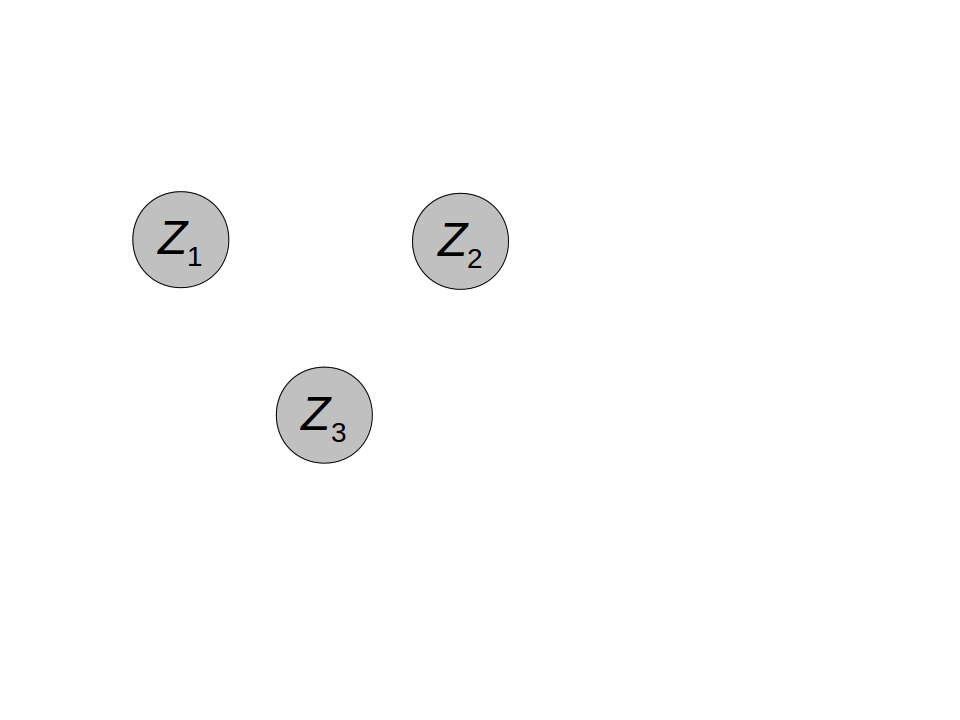
\includegraphics[width=0.6\textwidth]{../FIGURES/FigSBM-Z}
%        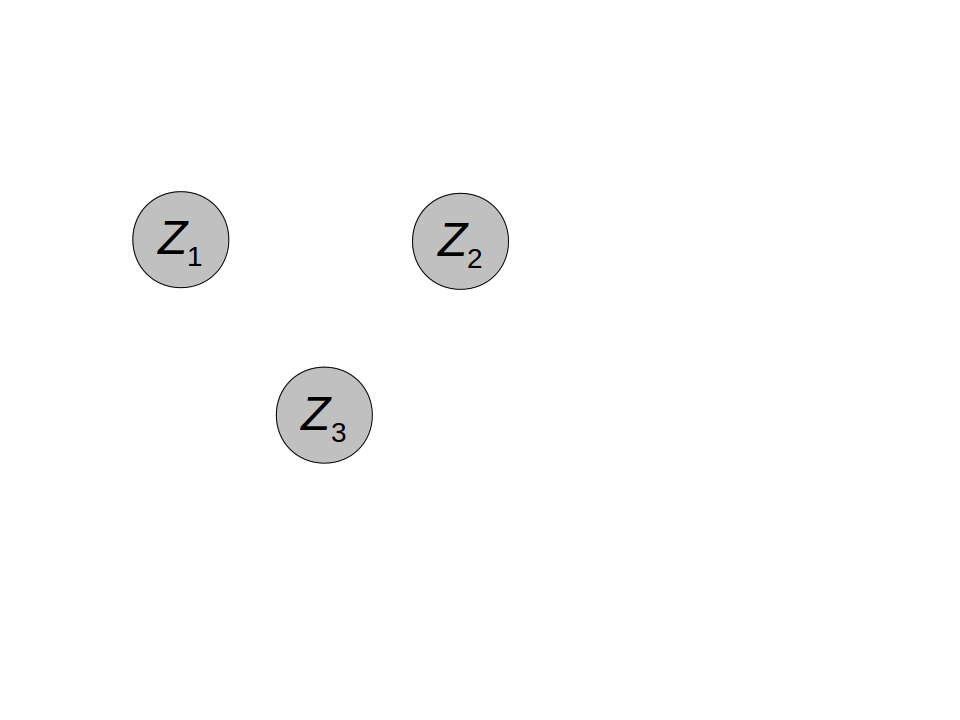
\epsfig{file=../FIGURES/FigSBM-Z.eps, clip=, width=0.6\textwidth}
        \onslide<3>
        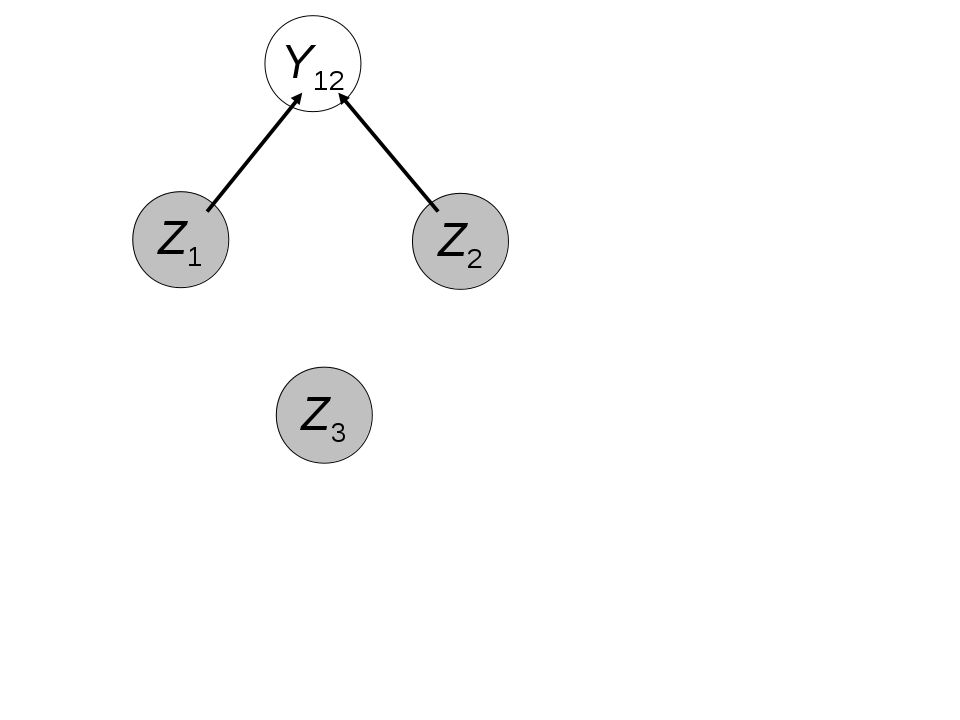
\includegraphics[width=0.6\textwidth]{../FIGURES/FigSBM-Z-Y12}
%         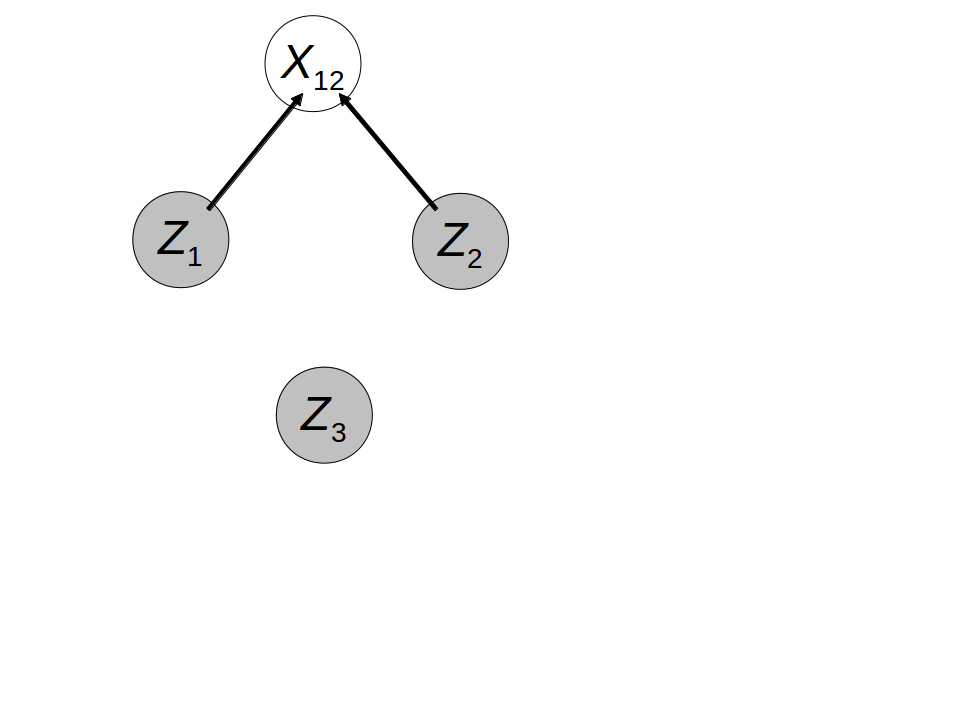
\epsfig{file=../FIGURES/FigSBM-Z-X12.eps, clip=, width=0.6\textwidth}
        \onslide<4>
        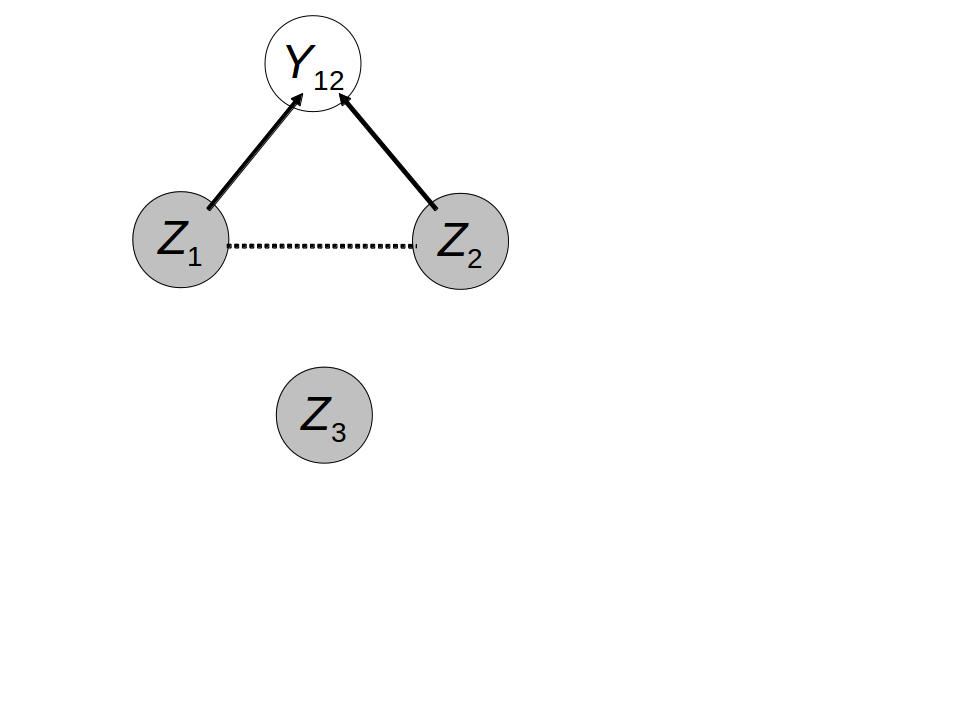
\includegraphics[width=0.6\textwidth]{../FIGURES/FigSBM-Z-Y12-Moral} 
%         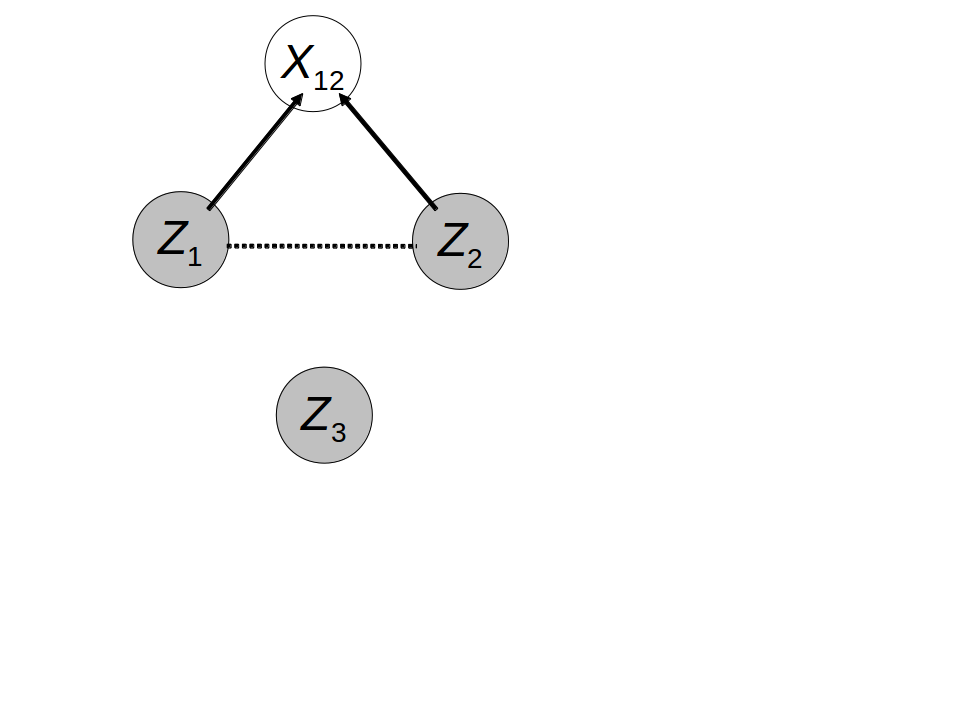
\epsfig{file=../FIGURES/FigSBM-Z-X12-Moral.eps, clip=, width=0.6\textwidth} 
        \onslide<5>
        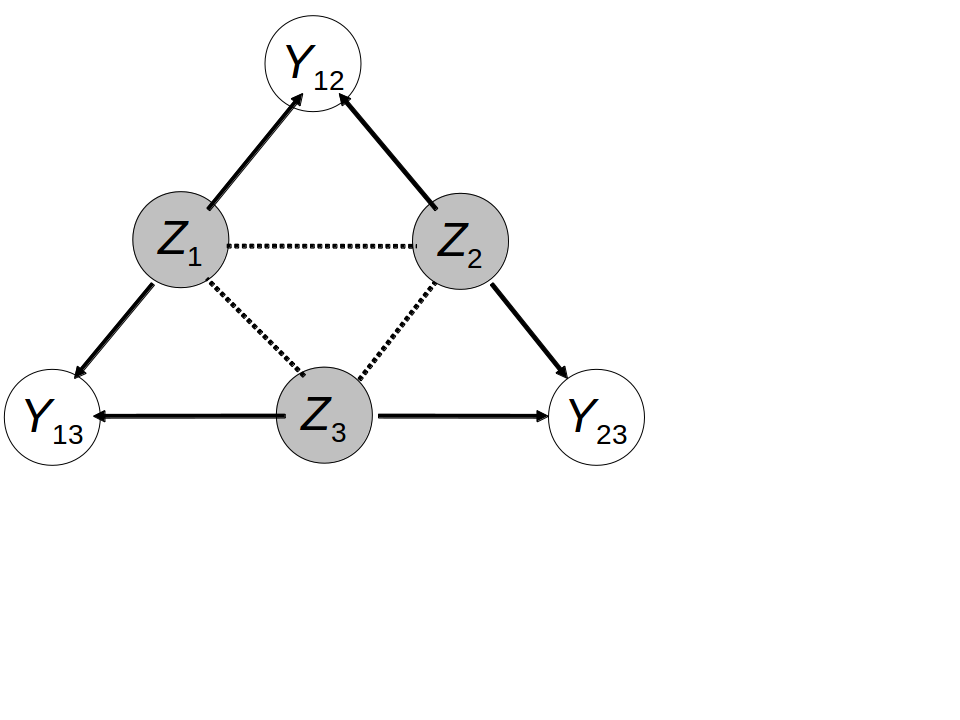
\includegraphics[width=0.6\textwidth]{../FIGURES/FigSBM-Z-Y-Moral} 
%         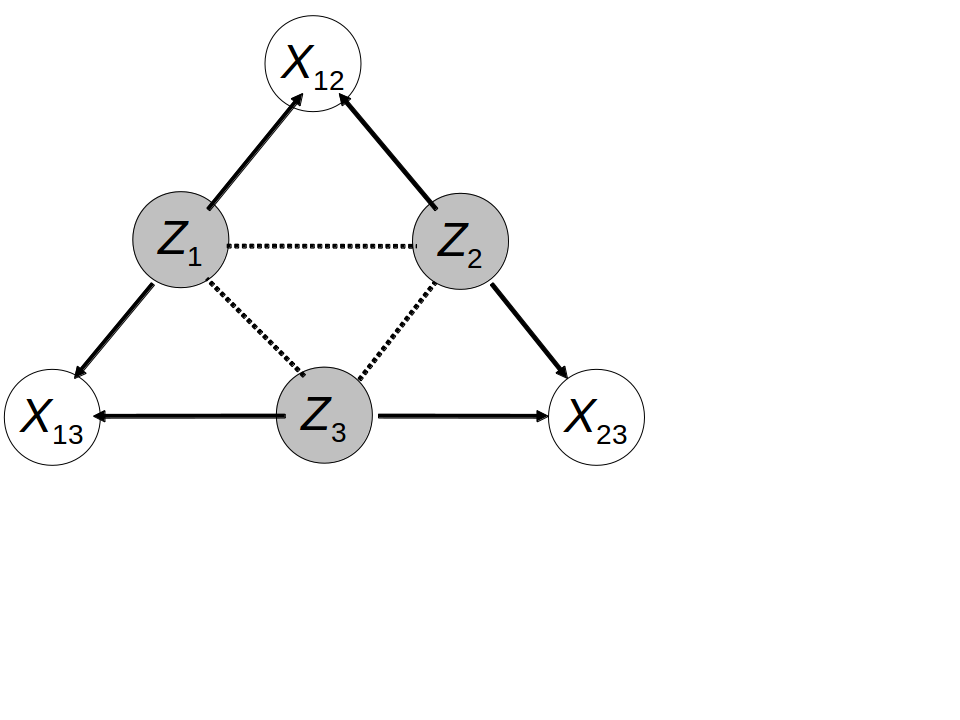
\epsfig{file=../FIGURES/FigSBM-Z-X-Moral.eps, clip=, width=0.6\textwidth} 
        \onslide<6->
        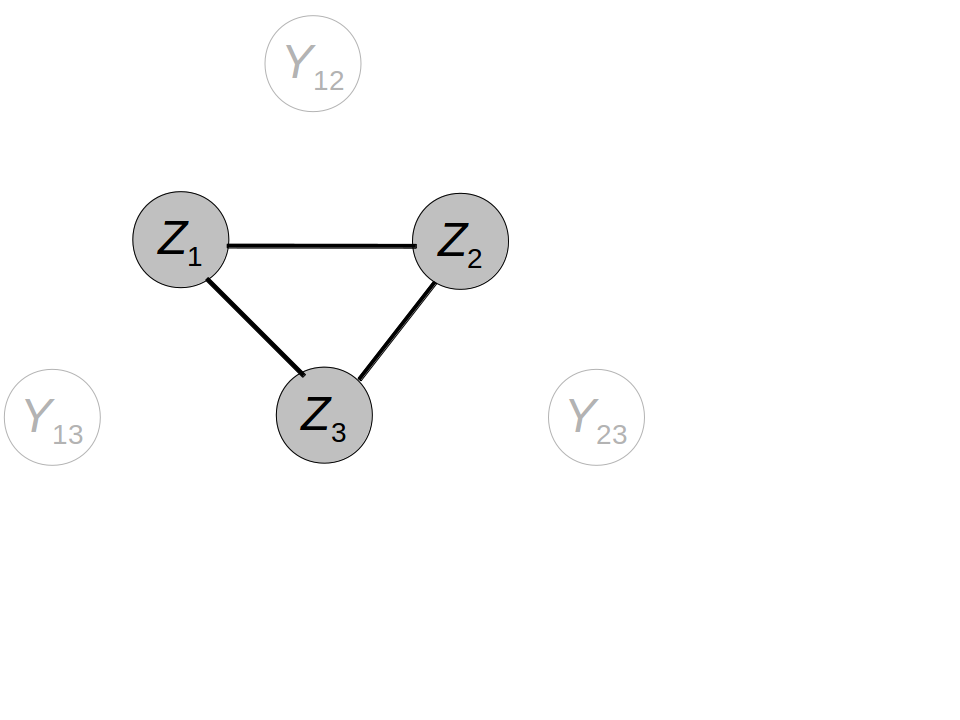
\includegraphics[width=0.6\textwidth]{../FIGURES/FigSBM-ZcondY}
%         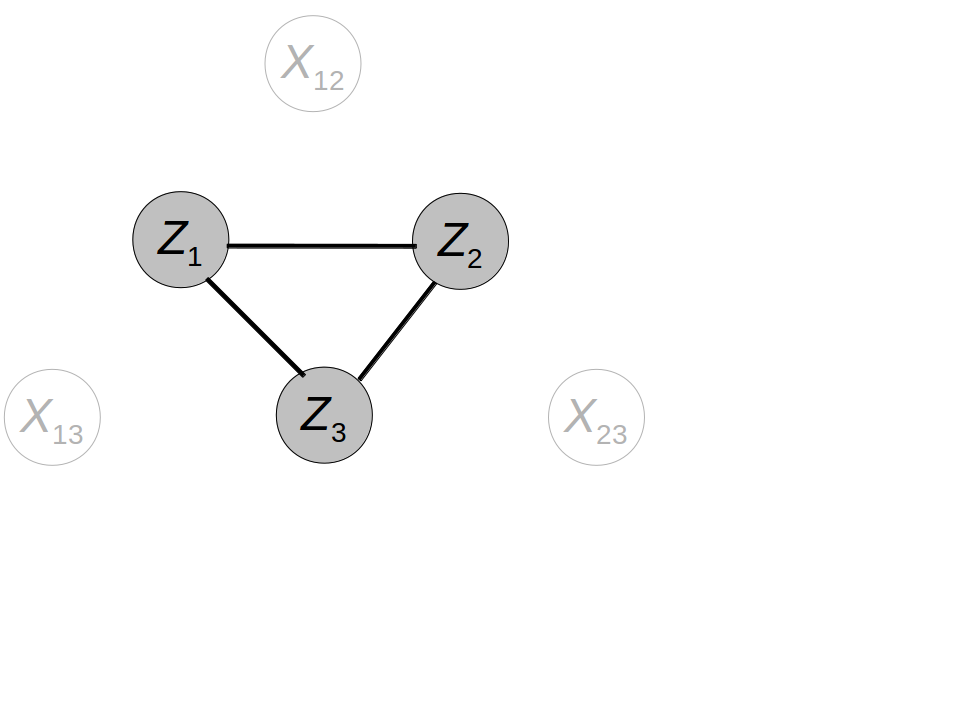
\epsfig{file=../FIGURES/FigSBM-ZcondX.eps, clip=, width=0.6\textwidth}
      \end{overprint}
    \end{tabular}
  \end{tabular}

  \onslide+<6->{
    \vspace{-1.5cm}
    \paragraph{Conditional distribution.} The dependency graph of
    $Z$ given $Y$ is a clique. \\
    \ra No factorization can be hoped (unlike for HMM). \\
    \ra $P(Z | Y; \theta)$ can not be computed
    (efficiently). \\
    \ra Variational techniques may help as they provide 
    $$
    Q(Z) \simeq P(Z | Y).
    $$
  }
}

%--------------------------------------------------------------------
\subsection*{Variational inference}
%--------------------------------------------------------------------
%--------------------------------------------------------------------
\frame{\frametitle{Variational inference}

  \paragraph{Lower bound of the log-likelihood.} For any distribution
  $Q(Z)$ \refer{Jaa00,WaJ08},
  \begin{eqnarray*}
    \log P(Y) & \geq & \log P(Y) - KL[Q(Z),
    P(Z|Y)] \\ 
%    & = & \log P(Y; \theta) - \int Q(Z) \log Q(Z) \dd Z
%    + \int
%    Q(Z) \log P(Z|Y) \\
%    & = & \log P(Y; \theta) - \int Q(Z) \log Q(Z) \dd Z
%    + \int
%    Q(Z) \log P(Y, Z) - \int Q(Z) \log P(Y) \dd Z \\ 
    & = & \int Q(Z) \log P(Y, Z) \dd Z - \int Q(Z) \log
    Q(Z) \dd Z \\ 
    & = & \Esp_Q[\log P(Y, Z)] + \Hcal[Q(Z)] 
  \end{eqnarray*}
  
  \bigskip\bigskip\pause
  \paragraph{Link with EM.} This is similar to
  $$
  \log P(Y) = \Esp[\log P(Y, Z)|Y] + \Hcal[P(Z | Y)]
  $$
  replacing $P(Z|Y)$ with $Q(Z)$.
  }
  
%--------------------------------------------------------------------
\subsection*{Variational EM}
%--------------------------------------------------------------------
\frame{\frametitle{Variational EM algorithm}

  \paragraph{Variational EM.} 
  \begin{itemize}
  \item M-step: compute 
    $$
    \widehat{\theta} = \arg\max_\theta \emphase{\Esp_{Q^*}}[\log P(Y,
    Z; \theta)].
    $$
  \item \pause E-step: replace the calculation of $P(Z|Y)$ with
    the search of
    $$
    Q^*(Z) = \emphase{\arg\min_{Q \in \Qcal} KL}[Q(Z), P(Z|Y)].
    $$ 
    \pause ~\\
    \ra Taking $\Qcal = \{\text{all possible distributions}\}$ gives $Q^*(Z) = P(Z|Y)$ ... like EM does. \\
    ~\\
   \ra Variational approximations rely on the choice of a 'good' and 'tractable' distribution set $\Qcal$.
  \end{itemize}

  }


  
%-------------------------------------------------------------------- 
\frame{ \frametitle{Variational EM for SBM}

  \paragraph{Distribution class.} $\Qcal =$ set of \emphase{factorisable}
  distributions:
  $$
  \Qcal = \{Q: Q(Z) = \prod_i Q_i(Z_i)\}, \qquad\qquad Q_i(Z_i) = \prod_k
  \tau_{ik}^{Z_{ik}}.
  $$
  \ra The approximate joint distribution is $Q(Z_i, Z_j) = Q_i(Z_i)
  Q_j(Z_j)$. 

  \bigskip \bigskip \pause
  The optimal approximation within this class satisfies a
  \emphase{fix-point} relation:
  $$
  \tau_{ik} \propto \pi_k \prod_{j \neq i} \prod_\ell
  f_{k\ell}(Y_{ij})^{\emphase{\tau_{j\ell}}}
  $$
  also known as  \emphase{mean-field approximation} in physics \refer{Par88}. 
  
  \bigskip \bigskip \pause
  \paragraph{Variational estimates.}
  \begin{itemize}
   \item No general statistical guaranty for variational estimates.
   \item SBM is a very specific case for which the variational approximation is asymptotically exact \refer{CDP12,MaM13}.
  \end{itemize}

  }

%--------------------------------------------------------------------
\subsection*{Variational Bayes EM}
%-------------------------------------------------------------------- 
\frame{ \frametitle{Variational Bayes inference}

  \vspace{-1.5cm}
  \begin{tabular}{cc}
    \hspace{-.5cm}
    \begin{tabular}{p{.4\textwidth}}  
	 \paragraph{Bayesian perspective.} \\
	 $\theta = (\pi, \gamma)$ is random. 
	 
	 \bigskip
	 \paragraph{Model:}
      \begin{itemize}
      \onslide+<2->{\item $P(\theta)$}
      \onslide+<3->{\item $P(Z|\pi)$}
      \onslide+<4->{\item $P(Y|\gamma, Z)$}
      \end{itemize}
      \vfill
    \end{tabular}
    & 
    %\hspace{-.5cm}
    \begin{tabular}{p{.6\textwidth}}
	 \vspace{1.3cm}
	 \begin{overprint}
	 \onslide<2>
	 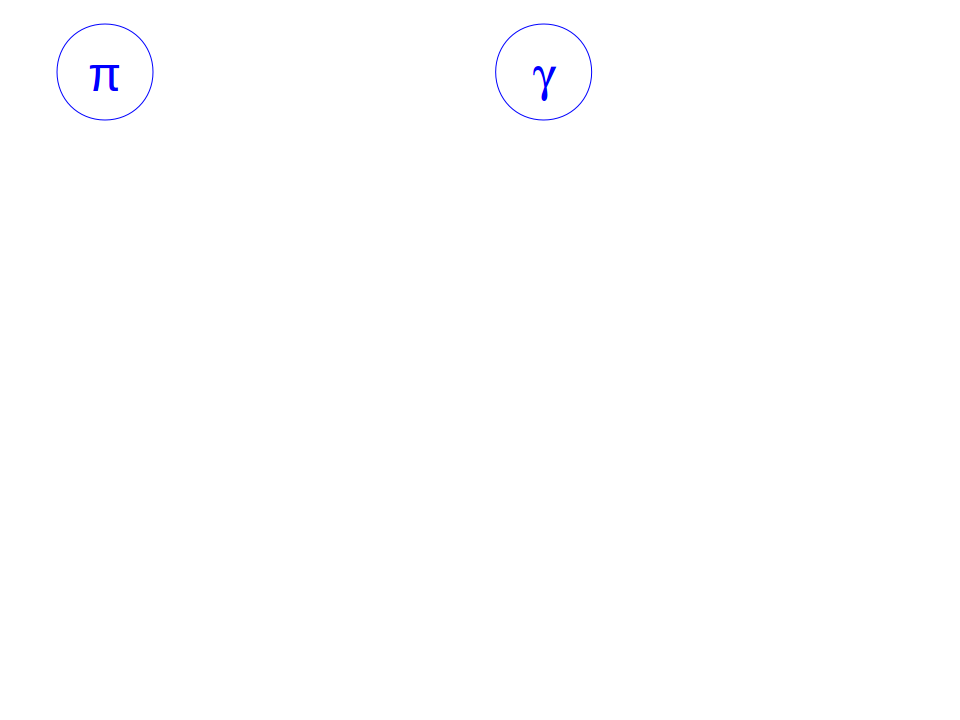
\includegraphics[width=.6\textwidth]{\fignet/FigSBM-Bayes-pi-gamma}    
	 \onslide<3>
	 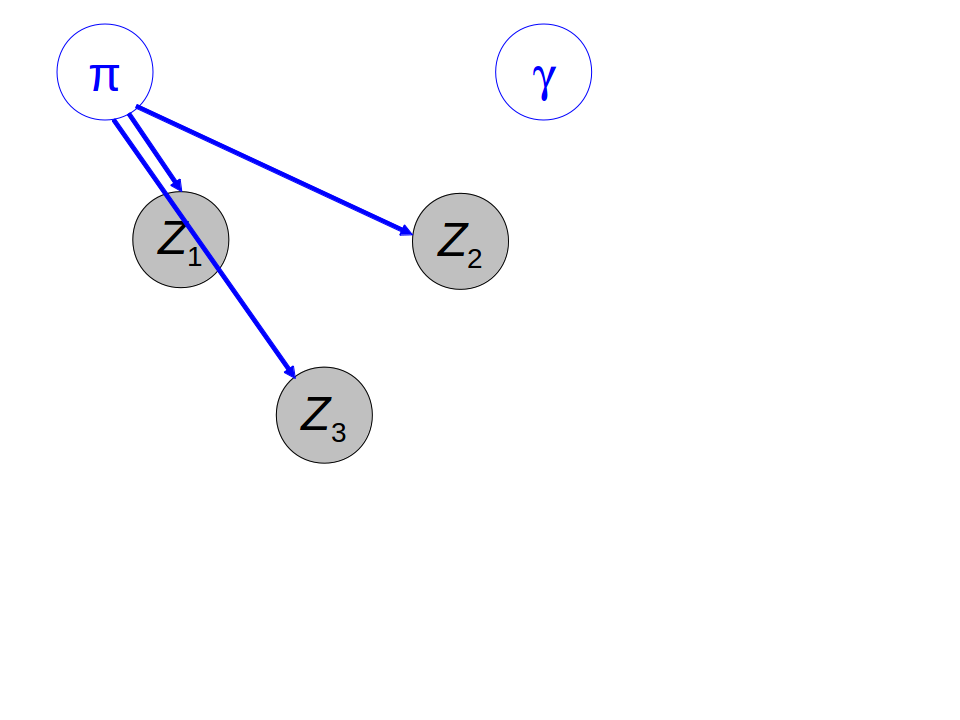
\includegraphics[width=.6\textwidth]{\fignet/FigSBM-Bayes-pi-gamma-Z}    
	 \onslide<4->
	 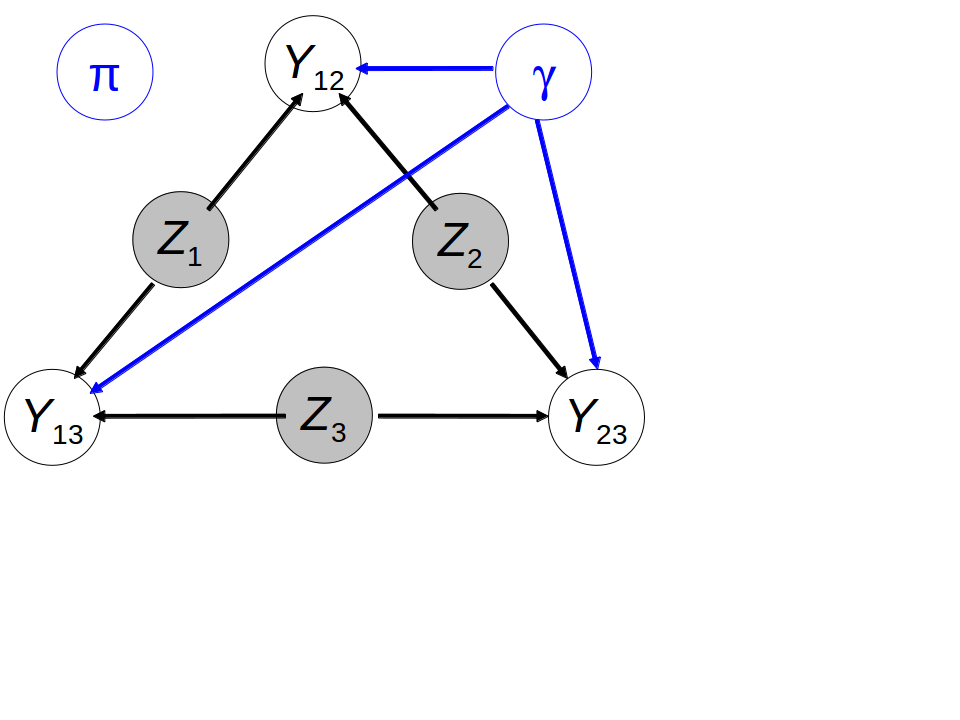
\includegraphics[width=.6\textwidth]{\fignet/FigSBM-Bayes-gamma-Z-Y}    
	 \end{overprint}
	 \vfill
    \end{tabular}
  \end{tabular}
  
  \vspace{-1cm} \pause
  \onslide+<5->{\paragraph{Bayesian inference.} The aim is then to get the joint conditional distribution of the parameters and of the hidden variables:
  $$
  P(\theta, Z |Y).
  $$}
  }

%-------------------------------------------------------------------- 
\frame{ \frametitle{Variational Bayes algorithm}

  \paragraph{Variational Bayes.} As $P(\theta, Z|Y)$ is intractable, one look formula
  $$
  Q^*(\theta, Z) = \arg\min_{Q \in \Qcal} KL\left[Q(\theta, Z) || P(\theta, Z|Y)\right]
  $$
  taking, e.g., $\Qcal = \{Q(\theta, Z) = Q_{\theta}(\theta) Q_Z(Z)\}$
  
  \bigskip \bigskip \pause
  \paragraph{Variational Bayes EM (VBEM)}. When
  \begin{itemize}
   \item $P(Z, Y | \theta)$ belongs to the exponential family, 
   \item $P(\theta)$ is the corresponding conjugate prior,
  \end{itemize}
  $Q^*$ can be obtained iteratively as \refer{BeG03} 
  $$
  \log Q_{\theta}^h(\theta) \propto \Esp_{Q^{h-1}_Z} \left[\log P(Z, Y, \theta)\right], 
  \quad
  \log Q_{Z}^h(Z) \propto \Esp_{Q^h_{\theta}} \left[\log P(Z, Y, \theta)\right].
  $$
%   \begin{itemize}
%    \item $\log Q_{\theta}^h \propto \Esp_{Q^{h-1}_Z} \log P(Z, Y, \theta)$ 
%    \item $\log Q_{Z}^h \propto \Esp_{Q^h_{\theta}} \log P(Z, Y, \theta)$ 
%   \end{itemize} 

  \pause \bigskip
  Application to SBM: \refer{LBA11b} 


}  

%--------------------------------------------------------------------
\subsection*{Illustration}
%--------------------------------------------------------------------
\frame{ \frametitle{{\VBEM}: Simulation study}

  \paragraph{Credibility intervals:}   $\pi_1$: $+$,
  $\gamma_{11}$: \textcolor{red}{$\triangle$}, $\gamma_{12}$:
  \textcolor{blue}{$\circ$}, $\gamma_{22}$: \textcolor{green}{$\bullet$} 
  $$
  \includegraphics[width=1\textwidth]{../FIGURES/im-ICQ2-2-new} 
  $$

  \pause
  \emphase{Width of the posterior credibility intervals.}
  {$\pi_1$}, \textcolor{red}{$\gamma_{11}$},
  \textcolor{blue}{$\gamma_{12}$}, \textcolor{green}{$\gamma_{22}$}
  \\
  \includegraphics[width=1\textwidth]{../FIGURES/im-ICQ2-3} \\

 }

%--------------------------------------------------------------------
% %--------------------------------------------------------------------
% \section{SBM analysis of biological networks}
% \frame{\frametitle{SBM analysis of biological networks}
% 
%   Joint work with J.-J. Daudin, V. Miele, F. Picard
% 
% }
% %--------------------------------------------------------------------

%-------------------------------------------------------------------- 
\frame{ \frametitle{SBM analysis of {\sl E. coli} operon networks}

  \vspace{-0.5cm}
  \hspace{-0.5cm}
  \begin{tabular}{cc}         
    \begin{tabular}{p{0.45\textwidth}}
       \onslide+<1->{
	\vspace{-1cm}
        \includegraphics[width=.45\textwidth]{\fignet/im_EcoliVEM_2} \\
          %~\\
          \refer{PMD09}
         }
    \end{tabular}
    &
    \begin{tabular}{p{0.45\textwidth}}
     \onslide+<2->{
      \vspace{-.3cm}
      \paragraph{Meta-graph representation.} \\
      %\vspace{-.5cm}
      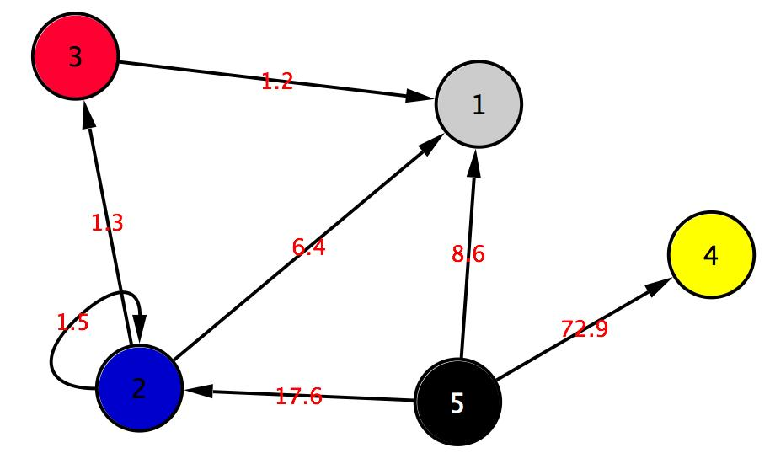
\includegraphics[width=.35\textwidth]{\fignet/VEMmetagraphe}  \\
     }
     \onslide+<3->{
      \vspace{-.3cm}
      \paragraph{Parameter estimates.} $K = 5$     \\
      \includegraphics[width=.35\textwidth]{../FIGURES/im-pi1BVEM}\\        
      \includegraphics[width=.35\textwidth]{../FIGURES/im-pi2BVEM}\\
      \includegraphics[width=.35\textwidth]{../FIGURES/im-pi3BVEM}\\
      \includegraphics[width=.35\textwidth]{../FIGURES/im-pi4BVEM}\\
      \includegraphics[width=.35\textwidth]{../FIGURES/im-pi5BVEM}\\
      \hline 
      \includegraphics[width=.35\textwidth]{../FIGURES/im-alphaBVEM}\\
     }
    \end{tabular}
  \end{tabular}
  }

%-------------------------------------------------------------------- 
\section{{(Variational) Bayesian model averaging}}
%-------------------------------------------------------------------- 
\frame{ \frametitle{(Variational) Bayesian model averaging}


  Joint work with M.-L. Martin-Magniette, S. Volant

  \bigskip \bigskip 
  \refer{VMR12}
}

%-------------------------------------------------------------------- 
\frame{ \frametitle{Model choice}

  \paragraph{Model selection.} The number of classes $K$ generally needs to be estimated.
  \begin{itemize}
  \item In the frequentist setting, an approximate ICL criterion can be derived
  $$
  ICL = \Esp[\log P(Y, Z)|Y] - \frac12 \left\{\frac{K(K+1)}2 \log \frac{n(n-1)}2 - (K-1) \log n\right\}.
  $$
  \item In the Bayesian setting, exact versions of BIC and ICL criteria can be calculated as $$
  \log P(Y, K), \qquad \log P(Y, Z, K).
  $$
  (up to the variational approximation) \refer{LBA11b}
  \end{itemize}
  
  \pause \bigskip
  \paragraph{But,} in some applications, it may be useless or meaningless and model averaging may be preferred.
  }

%-------------------------------------------------------------------- 
\frame{ \frametitle{Bayesian model averaging (BMA)}

  \paragraph{General principle.} \refer{HMR99} 
  \begin{itemize}
   \item $\Delta$: a parameter that can be defined under a series of different models $\{\Mcal_K\}_K$.
   \item Denote $P_K(\Delta | Y)$ its posterior distribution under model $\Mcal_K$.
  \end{itemize}
  The posterior distribution of $\Delta$ can be averaged over all models as 
  $$
  P(\Delta | Y) = \sum_K P(\Mcal_K |Y) P_K(\Delta | Y)
  $$
  
  \pause \bigskip
  \paragraph{Remarks.} 
  \begin{itemize}
   \item $w_k = P(\Mcal_K|Y)$: weight given to model $\Mcal_K$ for the estimation of $\Delta$. \\ \medskip
   \item Calculating of $w_K$ is not easy, but variational approximation may help.
  \end{itemize}


  }

%-------------------------------------------------------------------- 
\frame{ \frametitle{Variational Bayesian model averaging (VBMA)}

  \paragraph{Variational Bayes formulation.}
  \begin{itemize}
   \item $\Mcal_K$ can be viewed as one more hidden layer
   \item Variational Bayes then aims at finding
   $$
   Q^*(K, \theta, Z) = \arg\min_{Q \in \Qcal}KL\left[Q(K, \theta, Z) || P(K, \theta, Z|Y) \right]
   $$
   with $\Qcal = \{Q(\theta, Z, K) = Q_{\theta}(\theta|K) Q_Z(Z|K) Q_K(K)\}$\footnote{No additional approximation w.r.t. the regular \VBEM.}
  \end{itemize}
  
  \bigskip \bigskip \pause
  \paragraph{Optimal variational weights:} 
  \begin{eqnarray*}
    Q_K^*(K) & \propto & P(K) \exp \{\log P(Y|K) - KL[Q^*(Z, \theta|K); P(Z, \theta|Y, K)]\} \\
    \\
    & = & \emphase{P(K|Y)} e^{-{KL[Q^*(Z, \theta|K); P(Z, \theta|Y, K)]}}.
  \end{eqnarray*}

}

%--------------------------------------------------------------------
\frame{\frametitle{VBMA: the recipe}

  \paragraph{For $K = 1 \dots K_{\max}$} 
  \begin{itemize}
  \item Use regular {\VBEM} to compute the approximate conditional posterior 
    $$     
    Q^*_{Z, \theta|K}(Z, \theta|K) = Q^*_{Z|K}(Z|K)
    Q^*_{\theta|K}(\theta|K);
    $$ 
  \item Compute the conditional lower bound of the log-likelihood
    $$     
    L_K = \log P(Y|K) - KL[Q^*(Z, \theta|K); P(Z, \theta|Y, K)].    
    $$
  \end{itemize}

  \bigskip\pause
  \paragraph{Compute the approximate posterior of model $\Mcal_K$:} 
  $$
  w_K := Q_K(K) \propto P(K) \exp(L_K).
  $$ 

  \bigskip\pause
  \paragraph{Deduce the approximate posterior of $\Delta$:} 
  $$
  P(\Delta | Y) \approx \sum_K w_K Q^*_{\theta | K}(\Delta | K)
  $$
  }

%--------------------------------------------------------------------
%--------------------------------------------------------------------
\section{Towards $W$-graphs}
\frame{\frametitle{Towards $W$-graphs}

  Joint work with P. Latouche.

  \bigskip \bigskip 
  \refer{LaR13}
}
%--------------------------------------------------------------------

%--------------------------------------------------------------------
\frame{ \frametitle{$W$-graph model}

  \begin{tabular}{cc}
    \hspace{-.5cm}
    \begin{tabular}{p{.5\textwidth}}
	 \paragraph{$W$ graph.} ~\\
	 Latent variables:
	 $$
	 (Z_i) \text{ iid } \sim \Ucal_{[0, 1]},
	 $$
	 Graphon function $\gamma$:
	 $$
	 \gamma(z, z'): [0, 1]^2 \rightarrow [0, 1]
	 $$    
	 Edges:
	 $$
	 \Pr\{Y_{ij} = 1\} = \gamma(Z_i, Z_j)
	 $$    
	 \end{tabular}
    & 
    \hspace{-.1\textwidth}
    \begin{tabular}{p{.5\textwidth}}
	 Graphon function $\gamma(z, z')$ \\
      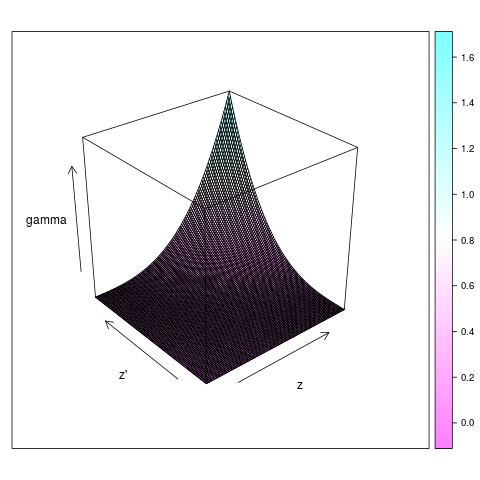
\includegraphics[width=.6\textwidth]{../FIGURES/FigCLADAG-W-graphon} \\
%       \includegraphics[width=.6\textwidth]{../FIGURES/FigGraphon-W-graphon} \\
    \end{tabular}
  \end{tabular}

 }


%--------------------------------------------------------------------
\frame{ \frametitle{Inference of the graphon function}

  \paragraph{Probabilistic point of view.}
  \begin{itemize}
   \item $W$-graph have been mostly studied in the probability literature: \refer{LoS06}, \refer{DiJ08}
   \item Motif (sub-graph) frequencies are invariant characteristics of a $W$-graph.
   \item Intrinsic un-identifiability of the graphon function $\gamma$ is often overcome by imposing that $u \mapsto \int \gamma(u, v) \dd v$ is monotonous increasing.
  \end{itemize}

  \bigskip \bigskip \pause
  \paragraph{Statistical point of view.}
  \begin{itemize}
   \item Not much attention has been paid to its inference until very recently: \refer{Cha12}, \refer{ACC13}, \refer{WoO13}, ...
   \item The two latter also uses SBM as a proxy for $W$-graph.
  \end{itemize}
}

%--------------------------------------------------------------------
\frame{ \frametitle{SBM as a $W$-graph model}

  \begin{tabular}{cc}
    \hspace{-.5cm}
    \begin{tabular}{p{.5\textwidth}}
	 Latent variables:
	 $$
	 (U_i) \text{ iid } \sim \Ucal[0, 1]
	 $$
	 $$
	 Z_{ik} = \Ibb\{\sigma_{k-1} \leq U_i < \sigma_k\}
	 $$ 
	 where $\sigma_k = \sum_{\ell = 1}^k \pi_{\ell}$.\\ ~
	 
	 Blockwise constant graphon:
	 $$
	 \gamma(z, z') = \gamma_{k\ell}
	 $$    
	 Edges:
	 $$
	 \Pr\{Y_{ij} = 1\} = \gamma(Z_i, Z_j)
	 $$    
	 \end{tabular}
    & 
    \hspace{-.1\textwidth}
    \begin{tabular}{p{.5\textwidth}}
	 Graphon function $\gamma^{SBM}_K(z, z')$ \\
%       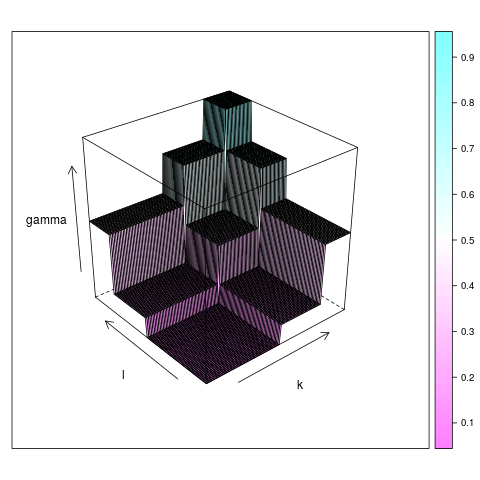
\includegraphics[width=.6\textwidth]{../FIGURES/FigCLADAG-SBM-graphon} \\
      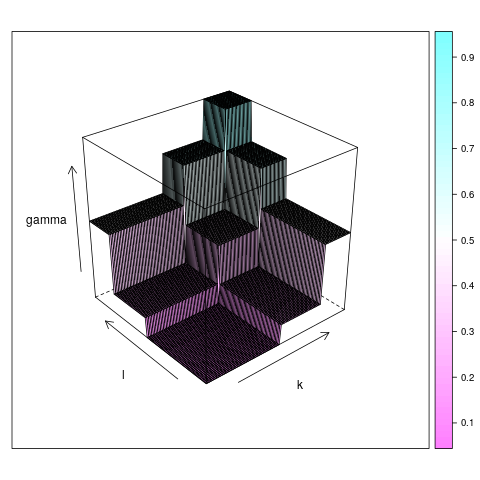
\includegraphics[width=.6\textwidth]{../FIGURES/FigGraphon-SBM-graphon} \\
    \end{tabular}
  \end{tabular}

 }

%--------------------------------------------------------------------
\subsection*{Variational Bayes inference}
%--------------------------------------------------------------------
\frame{ \frametitle{Variational Bayes estimation of $\gamma(z, z')$}

%   \paragraph{General idea.} Estimate the true $\gamma$ with a blockwise constant function $\gamma_K^{SBM}$ with $K$ classes.

  \begin{tabular}{cc}
    \hspace{-.5cm}
    \begin{tabular}{p{.5\textwidth}}
    \paragraph{VBEM inference} provides the approximate posteriors:
    \begin{eqnarray*}
    (\pi | Y) & \approx & \text{Dir}(\pi^*) \\
    (\gamma_{k\ell} | Y) & \approx & \text{Beta}(\gamma^{0*}_{k\ell}, \gamma^{1*}_{k\ell}) 
    \end{eqnarray*}
    ~
    
    \paragraph{Estimate of $\gamma(u, v)$.} 
    $$
    \widehat{\gamma}_K^{SBM}(u, v) = \widetilde{\Esp}\left(\gamma_{C(u), C(v)} | Y\right)
    $$
    where $C(u) = 1 + \sum_k \Ibb\{\sigma_k \leq u\}$. \\ ~
    \\
    \refer{GoS10}
    \end{tabular}
    & 
    \hspace{-.1\textwidth}
    \begin{tabular}{p{.5\textwidth}}
	 Posterior mean of $\gamma^{SBM}_K(z, z')$ \\
    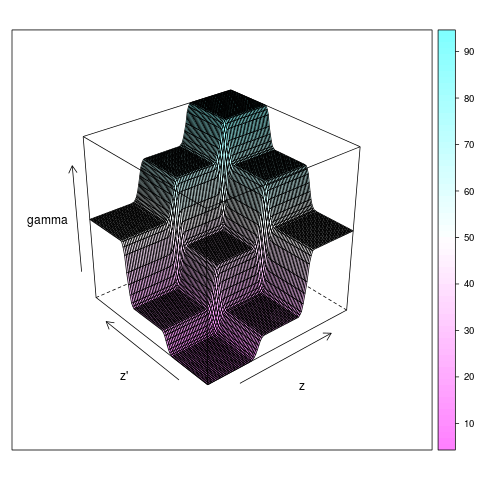
\includegraphics[width=.6\textwidth]{../FIGURES/FigGraphon-SBM-average} \\
    \end{tabular}
  \end{tabular}
  
}

%--------------------------------------------------------------------
\frame{ \frametitle{Model averaging}

  \paragraph{Model averaging:} There is no 'true $K$' in the $W$-graph model.

  \bigskip \bigskip 
  \paragraph{Apply VBMA recipe.}
  For $K = 1 .. K_{\max}$, fit an SBM model via VBEM and compute
  $$
  \widehat{\gamma}_K^{SBM}(z, z') = \Esp_Q[\gamma_{C(z), C(z')}].
  $$
  \pause 
  Perform model averaging as
  $$
  \widehat{\gamma}(z, z') = \sum_K w_K \widehat{\gamma}_K^{SBM}(z, z')
  $$
  where $w_K$ is the variational weights arising from variational Bayes inference.
%   \end{itemize}

}

%--------------------------------------------------------------------
\frame{ \frametitle{Some simulations}

  \begin{tabular}{cc}
    \hspace{-.5cm}
    \begin{tabular}{p{.5\textwidth}}
    \paragraph{Design.} Symetric graphon:
    $$
    \gamma(u, v) = \rho \lambda^2 (uv)^{\lambda-1}
    $$
    \begin{itemize}
     \item $\lambda \uparrow$: imbalanced graph 
     \item $\rho \uparrow$: dense graph
    \end{itemize}
    
    \bigskip
    \paragraph{Results.}
    \begin{itemize}
     \item More complex models \\
     as $n$ and $\lambda$ $\uparrow$
     \item Posterior fairly concentrated
    \end{itemize}

    \end{tabular}
    & 
    \hspace{-.1\textwidth}
    \begin{tabular}{p{.5\textwidth}}
    Variational posterior for $K$: $Q^*(K)$.
    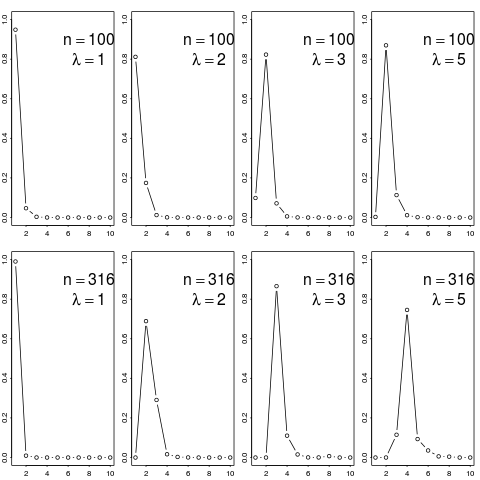
\includegraphics[width=.5\textwidth]{../FIGURES/PostDistQ-Talk-Lambda-N-rho0316227766016838}
    \end{tabular}
  \end{tabular}

}

%--------------------------------------------------------------------
\frame{ \frametitle{French political blogosphere}

  \paragraph{Website network.} French political blogs: 196 nodes, 1432 edges.
  $$
  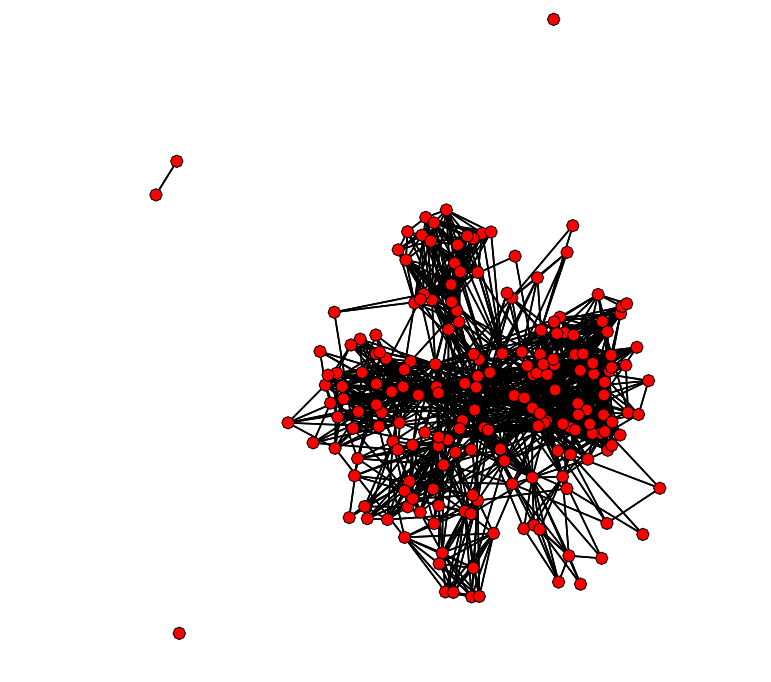
\includegraphics[width=.65\textwidth]{../FIGURES/Blogosphere-raw}
  $$
}

%--------------------------------------------------------------------
\frame{ \frametitle{French political blogosphere}

  \paragraph{Infered graphon.} $\widehat{W}(u, v) = \Esp(\gamma(u, v) | Y)$
  \begin{overprint}
  \onslide<1>
  \begin{center}
  \includegraphics[width=.5\textwidth]{../FIGURES/Blogosphere-contour}
  \end{center}
  \onslide<2->
  \begin{center}
  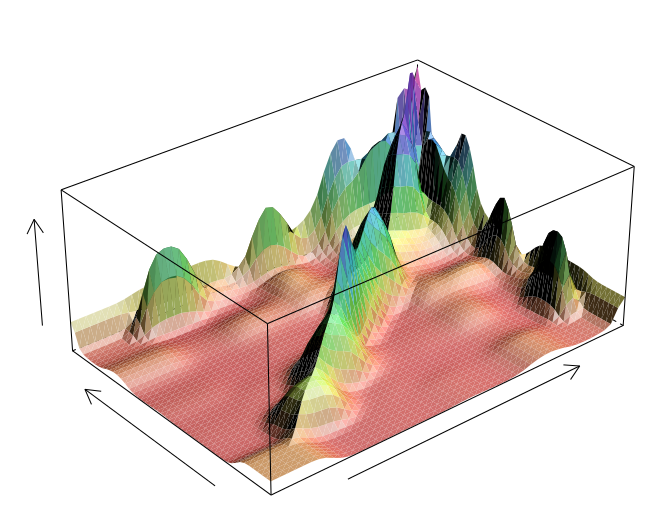
\includegraphics[width=.65\textwidth]{../FIGURES/Blogosphere-graphon}
  \end{center}
  \end{overprint}
  Motif probability can be estimated as well as $\widehat{\mu}(m) = \Esp(\mu(m) | Y)$.
}

%--------------------------------------------------------------------
\frame{\frametitle{Conclusion}

  \begin{itemize}
  \item Real networks are heterogeneous. \\ \pause ~
  \item State space models (including SBM) allow to capture such an heterogeneity ... 
  but raise inference problems. \\ \pause ~
  \item Variational approximations help to deal with complex (conditional) dependency structures. \\ \pause ~
  \item SBM is a special (rare?) case for which guaranties exist as for the performances of the variational approximation. \\ \pause ~
  \item SBM can be used as a proxy for smoother models, such as $W$-graphs.
  \end{itemize}
  }

%--------------------------------------------------------------------
{\tiny
  \bibliography{/home/robin/Biblio/ARC,/home/robin/Biblio/AST}%,/home/robin/Biblio/SSB}
  \bibliographystyle{/home/robin/LATEX/astats}
  %\bibliographystyle{plaine}
  }

%-------------------------------------------------------------------- 
\appendix
%-------------------------------------------------------------------- 
\frame{ \frametitle{SBM for a binary social network}

 \vspace{-.02\textheight}
 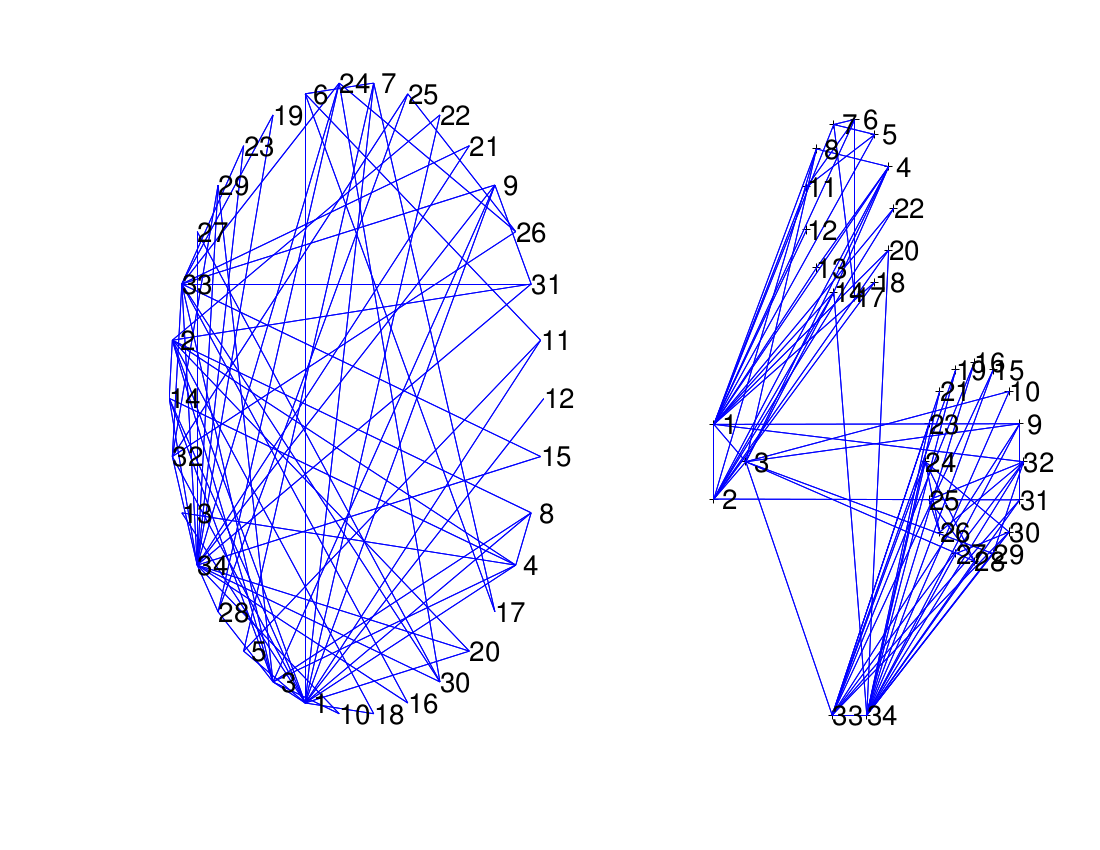
\includegraphics[width=.9\textwidth, height=.5\textheight]{\fignet/Karate-Graph}

%   \vspace{-.5cm}
  \begin{tabular}{ll}
    \begin{tabular}{p{.4\textwidth}}
    \paragraph{Zachary data.} Social binary network of friendship
    within a sport club. \\ 
    \\ 
%     \paragraph{Results.} 
%     The split is recovered and the role of few leaders is
%     underlined. 
    \end{tabular}
    & 
    \begin{tabular}{p{.5\textwidth}}
%     $
%     (Y_{ij}|Z_i=q, Z_j=\ell) \sim \Bcal(\gamma_{q\ell})
%     $ \\ ~\\
    {\small
    \begin{tabular}{c|rrrr}
    (\%) & \multicolumn{4}{c}{$\widehat{\gamma}_{k\ell}$} \\
    $k / \ell$ &  {1} & 2 & 3 &  4 \\
    \hline
    {1} &  {100} &   {53} &  {16} & {16} \\  
    {2} & - &  {12} & {0} & {7}  \\  
    3 & - & - & 8 & 73 \\
    4 & - & - & - & 100\\
    \hline
    $\widehat{\pi}_{\ell}$        & 9 &  38       & 47    & 6     \\
	 \end{tabular}}
    \end{tabular}
  \end{tabular}

}

%--------------------------------------------------------------------
\frame{\frametitle{K�llback-Leibler divergence}

  \paragraph{Definition.}
  \begin{eqnarray*}
    KL[Q(\cdot), P(\cdot)] & = & \int Q(Z) \log
    \frac{Q(Z)}{P(Z)} \dd Z \\
    & = & \int Q(Z) \log Q(Z) \dd Z - \int Q(Z) \log
    P(Z) \dd Z  
  \end{eqnarray*}

  \bigskip\bigskip%\pause
  \paragraph{Some properties.}
  \begin{itemize}
  \item Always positive.
  \item Null iff $P = Q$.
  \item Contrast consistent with maximum-likelihood inference.
  \item Not a distance, only a 'divergence'.
  \end{itemize}
  }

%-------------------------------------------------------------------- 
\frame{ \frametitle{Concentration of the degree distribution} 

  \begin{overprint}
   \onslide<1>
   \paragraph{$n = 100$.}
  $$
  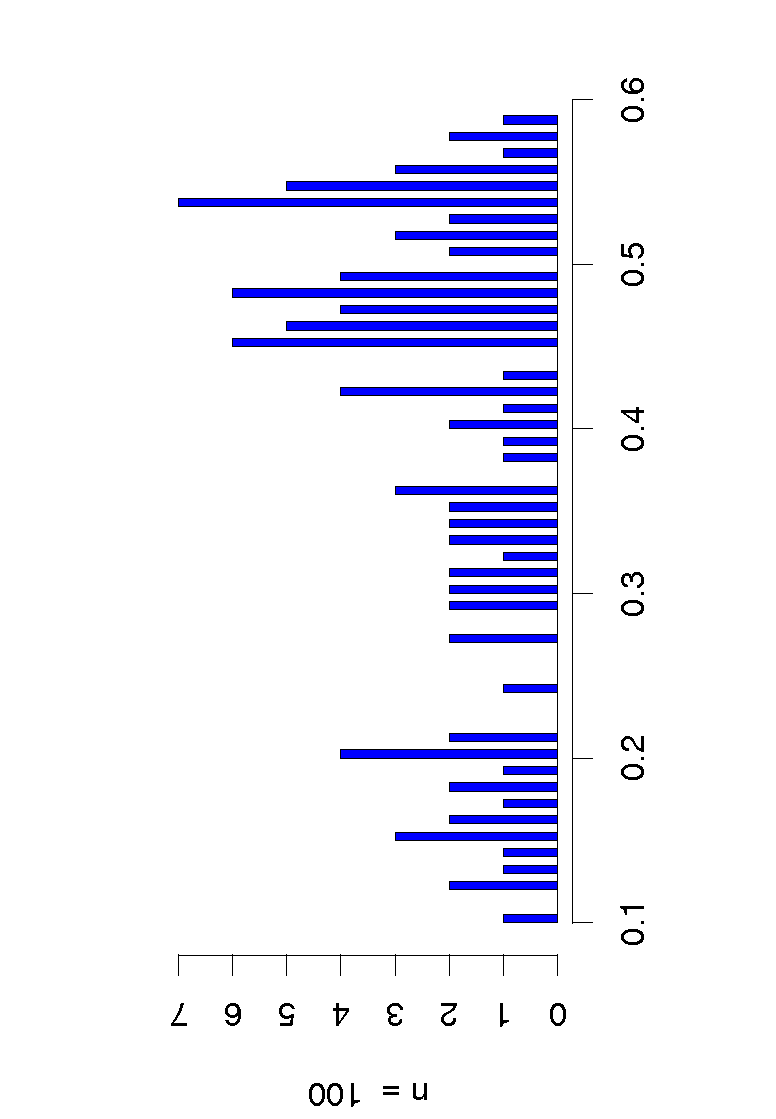
\includegraphics[width=.5\textwidth, angle=270]{\fignet/ConcentrBinom-n100}
  $$
   \onslide<2>
   \paragraph{$n = 1000$.}
  $$
  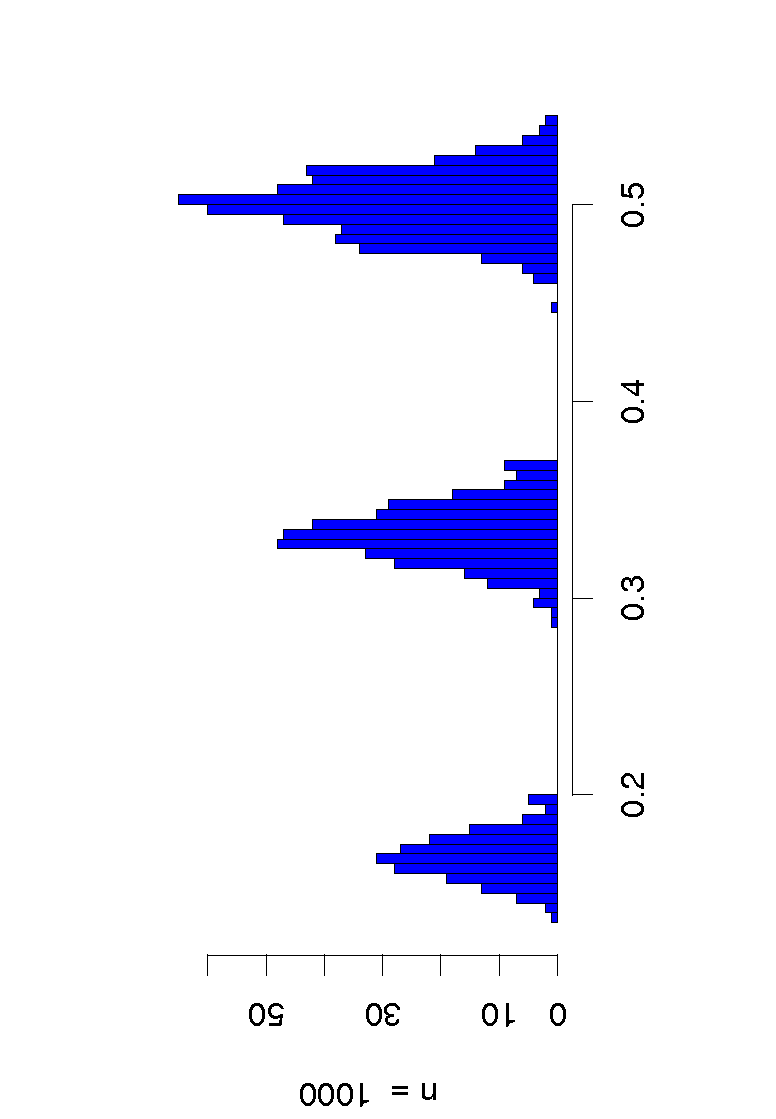
\includegraphics[width=.5\textwidth, angle=270]{\fignet/ConcentrBinom-n1000}
  $$
   \onslide<3>
   \paragraph{$n = 10000$.}
  $$
  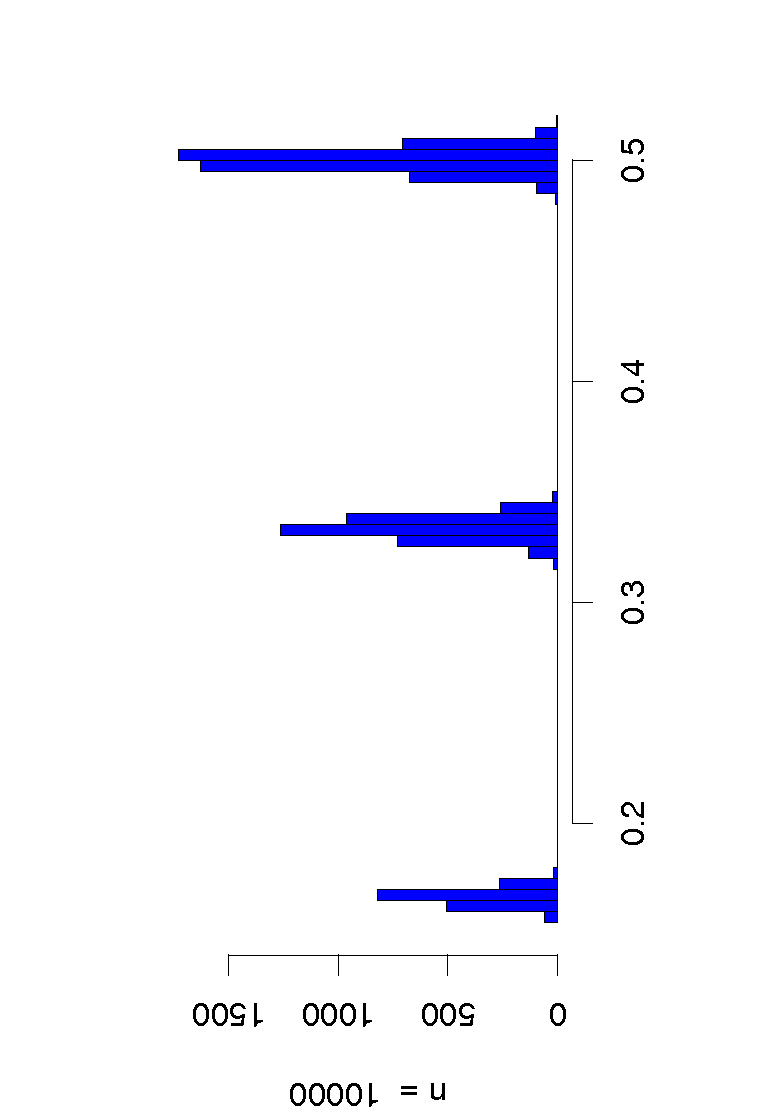
\includegraphics[width=.5\textwidth, angle=270]{\fignet/ConcentrBinom-n10000}
  $$
  \end{overprint}
  }
  


%--------------------------------------------------------------------
%--------------------------------------------------------------------
\end{document}
%--------------------------------------------------------------------
%--------------------------------------------------------------------

  \begin{tabular}{cc}
    \hspace{-.5cm}
    \begin{tabular}{p{.5\textwidth}}
    \end{tabular}
    & 
    \hspace{-.5cm}
    \begin{tabular}{p{.5\textwidth}}
    \end{tabular}
  \end{tabular}

